\documentclass{standalone}
\usepackage{tikz}
\usetikzlibrary{calc}
\usepackage{pgfplots}
% \usepgfplotslibrary{colormaps}
% \pgfplotsset{
  % this *defines* a custom colormap ...
  % colormap={}{
  %   rgb255=(112,128,144)
  %   rgb255=(255,159,101)
  % },
% \pgfplotsset{compat=1.16}

\begin{document}
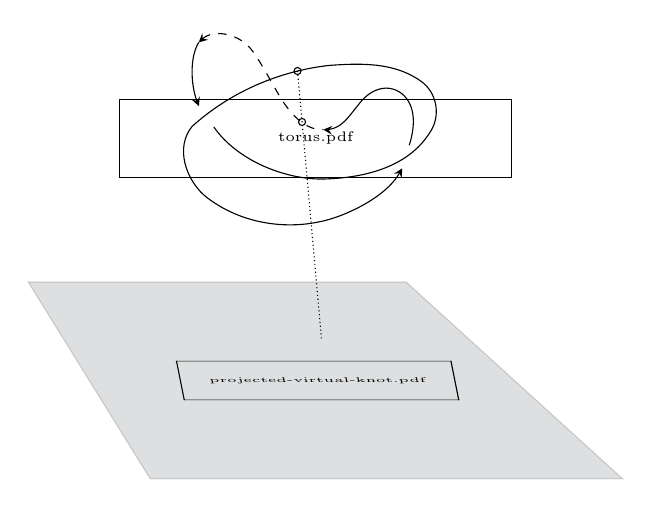
\begin{tikzpicture}
  % \pgfmathsetmacro{\rgbr}{214/255}
  % \pgfmathsetmacro{\rgbg}{215/255}
  % \pgfmathsetmacro{\rgbb}{217/255}
  \pgfmathsetmacro{\rgbr}{29/255}
  \pgfmathsetmacro{\rgbg}{37/255}
  \pgfmathsetmacro{\rgbb}{44/255}

  \draw[densely dotted, black] (2.245, -1.07) node (help) {} -- (2.55, -4.475);

  % \draw[white, opacity=.5] (2.75, -1) node (help) {} -- (2.55, -4.475);

  \definecolor{bmbfill}{rgb}{\rgbr,\rgbg,\rgbb}
  % \definecolor{drawcol}{rgb} {0.203,0.406,0.545}
  \definecolor{drawcol}{rgb} {0.0,0.0,0.0}
  \draw[draw=drawcol, dashed, stealth-, line width=0.4pt] (0.9901364013187068,
  -0.7061334563997764) .. controls (1.1893807958510865, -0.5264834245888681) and
  (1.5242412616399006, -0.6045285237810639) .. (1.6715943048834565,
  -0.8136513620852533) -- (1.6715943048834565, -0.8136513620852533) .. controls
  (1.8216181389654709, -1.021552348223409) and (1.9296011827874069,
  -1.2555765968111976) .. (2.0688030181804162, -1.4702828278933469) --
  (2.0688030181804162, -1.4702828278933469) .. controls (2.1847790105843568,
  -1.6375080732229272) and (2.351166086679905, -1.8232233848734314) ..
  (2.572774441381172, -1.8147580925022655);

  % Circles

  \pgfmathsetmacro{\myt}{.19}
  \pgfmathsetmacro{\myothert}{1 - \myt}
  \coordinate (theend) at (2.55, -4.475);
  \coordinate (aaaaa) at ($\myothert*(help) + \myt*(theend)$);
  \node[circle, draw=black, inner sep=.9pt] () at (aaaaa) {};

  \pgfdeclareimage[width=5cm]{torus}{torus.pdf}
  \node () at (2.475,-1.925) {\pgfuseimage{torus}};

  \node[circle, draw=black, inner sep=.9pt] () at (help) {};



  \begin{scope}[yshift=-5cm, xshift=2cm, cm={2,0, -1.5, 1, (0,0)}]
    \pgfmathsetmacro{\bxl}{-1.75}
    \pgfmathsetmacro{\txl}{-.65}
    \pgfmathsetmacro{\txr}{1.75}
    \pgfmathsetmacro{\bxr}{1.25}

    % \pgfmathsetmacro{\nmax}{10}
    % \foreach \n in {0,1,...,\nmax}{
    %   \pgfmathsetmacro{\xt}{((\nmax - \n)/\nmax) * (\txr - \txl) - .75}
    %   \pgfmathsetmacro{\xb}{((\nmax - \n)/\nmax) * (\bxr - \bxl) - 1.75}

    %   \draw[ultra thin] (\xt, 1.25) -- (\xb, -1.25);
    % }

    \filldraw[fill=bmbfill, opacity=.15] (\bxl, -1.25) -- (\txl, 1.25) -- (\txr,
    1.25) -- (\bxr, -1.25) -- cycle;
  \end{scope}
  \pgfdeclareimage[width=3.5cm]{proj}{projected-virtual-knot.pdf}
  \begin{scope}[cm={1,0, -.1,.5,(0,0)}]
    \node[transform shape, rotate=0] () at (1.5,-10) {\pgfuseimage{proj}};
  \end{scope}





  \draw[-stealth, draw=drawcol, opacity=1, line width=0.4pt] (1.1819256444118837,
  -1.780052873585379) -- (1.1819256444118837, -1.780052873585379) .. controls
  (1.486659517245368, -2.221605510998863) and (2.1384019597447415,
  -2.472891322369817) .. (2.6422465730976112, -2.438621575507529) --
  (2.6422465730976112, -2.438621575507529) .. controls (3.1135037305519675,
  -2.418917368755905) and (3.6481595461643757, -2.2840312614471077) ..
  (3.9179189400219787, -1.8623278837070316) -- (3.9179189400219787,
  -1.8623278837070316) .. controls (4.073356918390561, -1.649254781275907) and
  (4.021514536621104, -1.3341148614779543) .. (3.7980542327787314,
  -1.1895471524417287) -- (3.7980542327787314, -1.1895471524417287) .. controls
  (3.4647204977925163, -0.9566624814436369) and (3.0334978503537764,
  -0.9703348821068462) .. (2.6454211571458868, -0.9989620968208371) --
  (2.6454211571458868, -0.9989620968208371) .. controls (2.004460756906823,
  -1.070521096415971) and (1.3829650176405945, -1.34175670920974) ..
  (0.9044306570398504, -1.775234942836762) -- (0.9044306570398504,
  -1.775234942836762) .. controls (0.6889740259114308, -2.042398638878714) and
  (0.8269567323449459, -2.441351770807226) .. (1.0603662592299832,
  -2.6494459600146523) -- (1.0603662592299832, -2.6494459600146523) .. controls
  (1.5382066118490814, -3.038498428733926) and (2.226557240355511,
  -3.125931192041489) .. (2.79727920337774, -2.903821164857622) --
  (2.79727920337774, -2.903821164857622) .. controls (3.101825512348416,
  -2.7841931114924137) and (3.4082751739960284, -2.595086178642349) ..
  (3.5747729857911277, -2.305653352676936);

  \draw[-stealth, draw=drawcol, opacity=1, line width=0.4pt] (3.663826659469047,
  -2.0119446827584877) -- (3.663826659469047, -2.0119446827584877) .. controls
  (3.726522103761399, -1.8190885210819565) and (3.7596025564402633,
  -1.5533438325396671) .. (3.604002872621412, -1.389415137172492) --
  (3.604002872621412, -1.389415137172492) .. controls (3.5230836337696894,
  -1.2998970242341281) and (3.3898118336578693, -1.2639822196302222) ..
  (3.2752282191675186, -1.302652138078621) -- (3.2752282191675186,
  -1.302652138078621) .. controls (3.167219341032216, -1.3341478773448492) and
  (3.080414602170854, -1.4131378328095778) .. (3.0153605718251755,
  -1.5023579594748306) -- (3.0153605718251755, -1.5023579594748306) .. controls
  (2.933491343577089, -1.5984099606701496) and (2.8407121787580256,
  -1.7484532427847075) .. (2.716867493107637, -1.792353501127841) --
  (2.716867493107637, -1.792353501127841) .. controls (2.690489502400278,
  -1.8033765833156603) and (2.609634126356784, -1.8170931336636524) ..
  (2.5727744413811724, -1.814758092502265);

  \draw[-stealth, draw=drawcol, opacity=1, line width=0.4pt] (0.9901364013187068,
  -0.7061334563997764) -- (0.9901364013187068, -0.7061334563997764) .. controls
  (0.8723901559698473, -0.9008295899284737) and (0.8909385422892288,
  -1.2491887495421157) .. (0.9919563708573522, -1.5162799070735895);


% \end{axis}
\end{tikzpicture}
\end{document}
